%%%%%%%%%%%%%%%%%%%%%%%%%%%%%%%%%%%%%%%%%
% Beamer Presentation
% LaTeX Template
% Version 1.0 (10/11/12)
%
% This template has been downloaded from:
% http://www.LaTeXTemplates.com
%
% License:
% CC BY-NC-SA 3.0 (http://creativecommons.org/licenses/by-nc-sa/3.0/)
%
%%%%%%%%%%%%%%%%%%%%%%%%%%%%%%%%%%%%%%%%%

%----------------------------------------------------------------------------------------
%	PACKAGES AND THEMES
%----------------------------------------------------------------------------------------

\documentclass[xcolor=table]{beamer}

\mode<presentation> {

% The Beamer class comes with a number of default slide themes
% which change the colors and layouts of slides. Below this is a list
% of all the themes, uncomment each in turn to see what they look like.

\usetheme{default}
%\usetheme{AnnArbor}
%\usetheme{Antibes}
%\usetheme{Bergen}
%\usetheme{Berkeley}
%\usetheme{Berlin}
%\usetheme{Boadilla}
%\usetheme{CambridgeUS}
%\usetheme{Copenhagen}
%\usetheme{Darmstadt}
%\usetheme{Dresden}
%\usetheme{Frankfurt}
%\usetheme{Goettingen}
%\usetheme{Hannover}
%\usetheme{Ilmenau}
%\usetheme{JuanLesPins}
%\usetheme{Luebeck}
%\usetheme{Madrid}
%\usetheme{Malmoe}
%\usetheme{Marburg}
%\usetheme{Montpellier}
%\usetheme{PaloAlto}
%\usetheme{Pittsburgh}
%\usetheme{Rochester}
%\usetheme{Singapore}
%\usetheme{Szeged}
%\usetheme{Warsaw}

% As well as themes, the Beamer class has a number of color themes
% for any slide theme. Uncomment each of these in turn to see how it
% changes the colors of your current slide theme.

%\usecolortheme{albatross}
%\usecolortheme{beaver}
%\usecolortheme{beetle}
%\usecolortheme{crane}
%\usecolortheme{dolphin}
%\usecolortheme{dove}
%\usecolortheme{fly}
%\usecolortheme{lily}
%\usecolortheme{orchid}
%\usecolortheme{rose}
%\usecolortheme{seagull}
%\usecolortheme{seahorse}
%\usecolortheme{whale}
%\usecolortheme{wolverine}
%\setbeamertemplate{footline} % To remove the footer line in all slides uncomment this line
\setbeamertemplate{footline}[page number] % To replace the footer line in all slides with a simple slide count uncomment this line

\setbeamertemplate{navigation symbols}{} % To remove the navigation symbols from the bottom of all slides uncomment this line 
}
\usepackage{amsmath} 
\usepackage{graphicx} % Allows including images
\usepackage{booktabs} % Allows the use of \toprule, \midrule and \bottomrule in tables
\usepackage[table]{xcolor}
\usepackage{pgfplots}
\usepackage{tcolorbox}
\pgfplotsset{compat=1.15}
\usepackage{mathrsfs}
\usetikzlibrary{arrows}
\usetikzlibrary{patterns}


\usepackage{tikz}
\usepackage{pstricks-add}
\usetikzlibrary{arrows,shapes,positioning,shadows,trees}


\usepackage{tcolorbox}
\usepackage{wrapfig}


\usepackage{hyperref}
\hypersetup{
    colorlinks,
    citecolor=black,
    filecolor=black,
    linkcolor=black,
    urlcolor=black
}
\newcommand{\notimplies}{%
    \mathrel{{\ooalign{\hidewidth$\not\phantom{=}$\hidewidth\cr$\implies$}}}}


\DeclareMathAlphabet\mathzapf{T1}{pzc}{mb}{it}
\usepackage{amsmath,wasysym}
\usepackage{latexsym}

\usepackage{amssymb}
\usepackage{mathrsfs}
\usepackage{bm}
\usepackage{wrapfig}
\usepackage{fancybox}
\bibliographystyle{amsplain}
\usepackage{systeme}
\usepackage{pdfpages}


\usepackage{yfonts}
\usepackage[french]{babel}



\usepackage[T2A]{fontenc}




%\usepackage[style=ieee]{biblatex} %Use if necessary for citation
%\addbibresource{biblatex-examples.bib}
%----------------------------------------------------------------------------------------
%	TITLE PAGE
%----------------------------------------------------------------------------------------

\title[Physique]{Mécanique I} % The short title appears at the bottom of every slide, the full title is only on the title page

\author{Team Physique} % Your name
\institute[S4S] % Your institution as it will appear on the bottom of every slide, may be shorthand to save space
{
initiative S4S\\ % Your institution for the title page
\medskip
}
\date{\today} % Date, can be changed to a custom date

\begin{document}

\begin{frame}
\titlepage % Print the title page as the first slide
\end{frame}

\begin{frame}{Référentiel}
    \begin{itemize}
        \item Référentiel: Objet physique par rapport auquel on évalue la position et le mouvement
        
        \item Première moitié du semestre: référentiel du sol terrestre
    \end{itemize}
    
    \vspace{0.5 cm}
    \begin{center}
         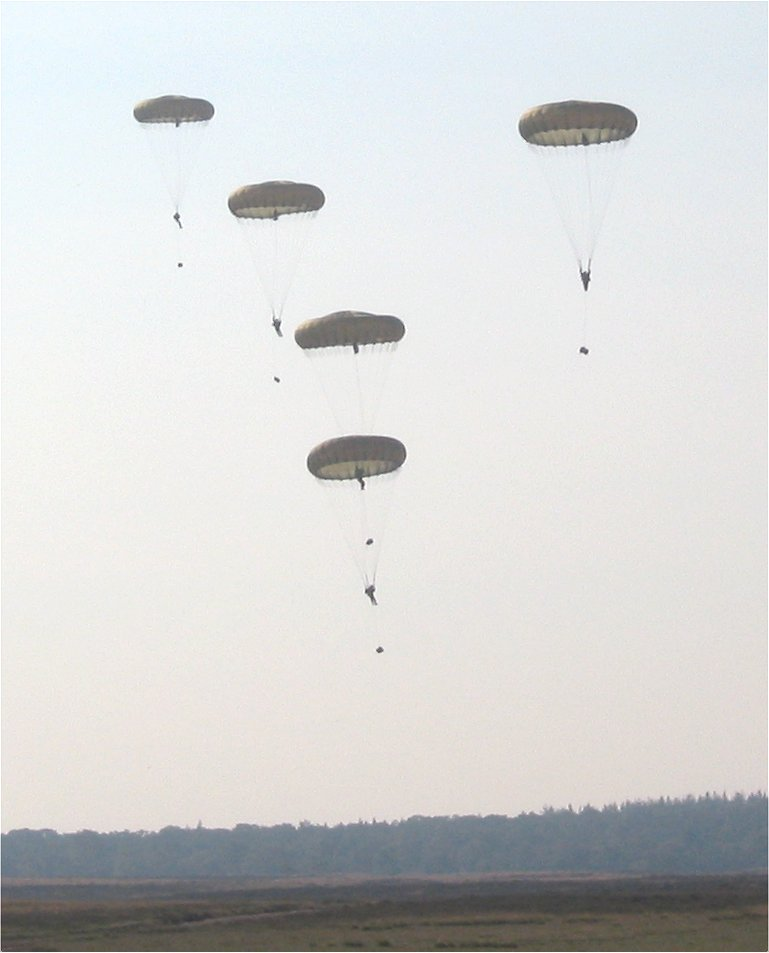
\includegraphics[scale = 0.25]{Images/Parachutisten.jpg} \hspace{1cm}
        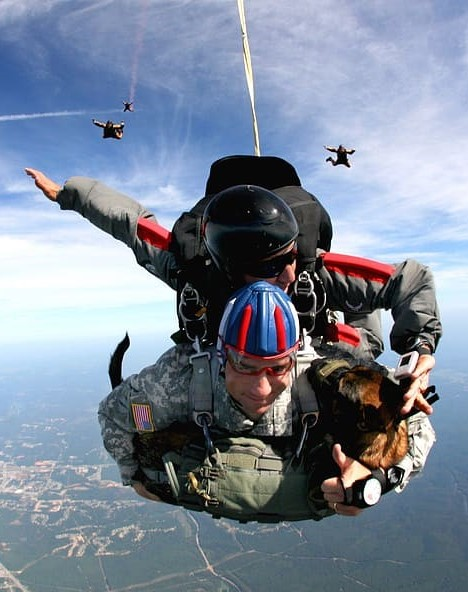
\includegraphics[scale = 0.21]{Images/skydiv2.jpg}
    \end{center}
   
\end{frame}

\begin{frame}{Repère}
\begin{itemize}
    \item Repère: Objet géométrique constitué d'une base orthonormée de vecteurs
    
    \item Permet d'identifier chaque point de l'espace avec un système de coordonnées
\end{itemize}
    
    
    %repere 2d
    \vspace{1cm}
  
  \begin{center}
    \begin{tikzpicture} [scale=0.7, every node/.style={scale=0.7}]
    \draw[line width=1.2pt,-latex,blue](0,0)--(3,0)node[midway,below]{$\vec{e}_x$};
    \draw[line width=1.0pt,-latex,green](0,0)--(0,3)node[pos=0.7,right]{$\vec{e}_z$};
    \end{tikzpicture} \hspace{1cm}
    \begin{tikzpicture} [scale=0.7, every node/.style={scale=0.7}]
    \draw[line width=1.2pt,-latex,blue](0,0)--(3,0)node[midway,below]{$\vec{e}_x$};
    \draw[line width=1.2pt,-latex,red](0,0)--(1,1)node[midway,above]{$\vec{e}_y$};
    \draw[line width=1.0pt,-latex,green](0,0)--(0,3)node[pos=0.7,right]{$\vec{e}_z$};
    \end{tikzpicture}
    \end{center}
\end{frame}

\begin{frame}{Repère : Fonctionnement}

\begin{center}
\begin{tikzpicture}[scale=2]
\draw [->,blue]  (0,0) -- (0:1);
\draw [->,blue]  (0:1) -- (0:2);
\draw [->,blue]  (0:2) -- (0:3);
%\draw [->,green]  (0,0) -- (90:1);
\draw [->,green]  (0:3) -- (3,1);
\draw [->,green]  (3,1) -- (3,2);
%\draw [->]  (0,0) -- (3,2);
\fill (3,2.05) circle (0.05);
\draw [->]  (0,0) -- (3,2);
\draw (0,0) node[below left]{$O$};
\draw (3,2.05) node[right]{$r(3;2)$};
\draw (3,1.0) node[right,green]{$2\vec e_y$};
\draw (1.5,0.0) node[below,blue]{$3\vec e_x$};
\draw (1.5,1.2) node[left]{$\vec r = 3\vec e_x + 2\vec e_y$};
\end{tikzpicture}    
\end{center}   
\end{frame}
\begin{frame}{Forces}
    Force: Action mécanique que génère un objet sur un autre. \\
    Notée $\vec{F}$, $[F]=N=\dfrac{m.kg}{s^2}$ 
\end{frame}


\begin{frame}{Forces: Exemples}
    \begin{itemize}
        \item Force de gravitation: $\vec{F} = -G\dfrac{m_1m_2}{d^2} \vec{e}_r$
        \item Poids : $\vec{P}=m\vec{g}= -G\dfrac{m.M_T}{R_T^2} \vec{e}_r$
        \item Force élastique $\vec{F_e} = -k \vec{d} = -k(x - x_0) \vec{e_r}$
    \end{itemize}
            \begin{figure}[h]
        \centering
        \begin{tikzpicture}
        \pgfmathsetmacro{\EqPos}{2}
        \pgfmathsetmacro{\Xmax}{3}
        \draw[dotted] (-1,\EqPos)--(5,\EqPos);

\node[circle,fill=purple,inner sep=2.5mm] (a) at (0,1) {};
\node[circle,fill=purple,inner sep=2.5mm] (b) at (4,2) {};
\node[circle,fill=purple,inner sep=2.5mm] (c) at (2,3) {};
\draw[decoration={aspect=0.3, segment length=3mm, amplitude=3mm,coil},decorate] (0,5) -- (a); 
\draw[decoration={aspect=0.3, segment length=1.5mm, amplitude=3mm,coil},decorate] (4,5) -- (b); 
\draw[decoration={aspect=0.3, segment length=1.5mm, amplitude=3mm,coil},decorate] (2,5) -- (c); 
\fill [pattern = north east lines] (-1,5) rectangle (5,5.2);
\draw[thick] (-1,5) -- (5,5);
\draw [-latex](a) -- (0,2);
\draw [-latex](c) -- (2,2);
\draw (5,2) node[right]{$x_0$};
\end{tikzpicture}
        \caption{Force élastique ($k=1)$}
        \label{fig:hooke}
    \end{figure}
\end{frame}

\begin{frame}{Quantité de Mouvement}
 \[\vec{p}=m\vec{v}\]
\begin{center}
    $m$ constante $\implies$ $\dfrac{d\vec{p}}{dt}=m \dfrac{d\vec{v}}{dt}=m\vec{a}$
\end{center} 

 %\par\leavevmode\par
  %  $\dot{\vec{p}}=0 \implies \vec{p}=cst$
\end{frame}

\begin{frame}{Lois de Newton: Première Loi}
    \textit{ "Tout corps dans un référentiel galiléen persévère dans un état de repos ou dans un mouvement rectiligne uniforme tant qu'aucune force ne s'exerce sur lui"}
\end{frame}

\begin{frame}{Lois de Newton: Deuxième Loi}
    \begin{equation*}
    \dfrac{d\vec p}{dt}=\sum \vec {F}^{ext}
\end{equation*}\\
\par\leavevmode\par
\par\leavevmode\par
Avec $m$ constante : $m\vec{a}=\sum \vec{F}^{ext}$
\end{frame}

\begin{frame}{Lois de Newton: Troisième Loi}
    \textit{"Tout corps A qui exerce une force sur un corps B subit une force d'intensité égale, de même direction mais dans un sens opposé"}
\end{frame}

\begin{frame}{Balistique : chute libre}
\vspace*{1cm}
\begin{center}
    

    \noindent\begin{minipage}{0.5\textwidth}
 \begin{figure}[H]
    \centering
    
\definecolor{uuuuuu}{rgb}{0.26666666666666666,0.26666666666666666,0.26666666666666666}
\begin{tikzpicture}[line cap=round,line join=round,>=triangle 45,x=1.0cm,y=1.0cm]
\draw [->] (0.05,0.1)--(0.05,1.1);
\draw (0.05,0.6) node[left]{$\vec e_x$};
\begin{axis}[
x=1.0cm,y=1.0cm,
axis y line=middle,
axis x line=none,
ymajorgrids=true,
xmajorgrids=false,
xmin=-0.05,
xmax=1.5,
ymin=-0.1,
ymax=7.0,
xtick={-0.0,2.0},
ytick={-0.0},]
\clip(-0.05,-0.1) rectangle (1.5,7.);
\draw[line width=0.8pt] (-2.8087273377408764,8.902841339382519) -- (0.17459772664676576,8.902841339382519);
\begin{scriptsize}
\draw [fill=black] (0.17459772664676576,8.902841339382519) circle (1.5pt);
\draw[color=black] (0.3237639798661478,9.193715533160313) node {$t = 1.2$};
\draw [fill=uuuuuu] (1.,-0.0032) circle (2.0pt);
\draw[color=uuuuuu] (1.0994284966069348,0.24374033999739933) node {$M$};
\draw[color=uuuuuu] (0.2,6.8) node {$x$};
\draw [fill=uuuuuu] (1.,6.8638) circle (2.0pt);
\draw [fill=uuuuuu] (1.,6.2752) circle (2.0pt);
\draw [fill=uuuuuu] (1.,5.2942) circle (2.0pt);
\draw [fill=uuuuuu] (1.,3.9208) circle (2.0pt);
\draw [fill=uuuuuu] (1.,2.155) circle (2.0pt);
\draw [fill=uuuuuu] (1.,-0.0032) circle (2.0pt);

\end{scriptsize}
\end{axis}
\draw [<-] (-1,4) -- (-1,5);
\draw (-1,4.5) node [left]{$\vec g$};
\end{tikzpicture}
    %\caption{Le point $M$ est en chute libre}
    \label{fig:my_label}
\end{figure}
\vspace{2\baselineskip}
\end{minipage}

%$m\vec a = m\vec \iff mx\vec e_x = -mg \vec e_x \iff m\ddot x = -mg $
\end{center}
\end{frame}
\begin{frame}{Balistique : Boulet de canon} 
Énoncé : Cela fait plusieurs semaines que vos voisins font du boucan tous les soirs, vous empêchant de réviser correctement votre examen de mécanique. Pour régler le conflit une bonne fois pour toutes, vous décidez d'acquérir un canon et de viser leurs enceintes. Vous connaissez la masse $m$ du boulet, la distance $d$ de votre cible et la vitesse $v_0$ initiale fourni par le canon. Problème: sauriez vous trouver l'angle (ou les angles) qui permettent d'atteindre la cible ?
\begin{center}
    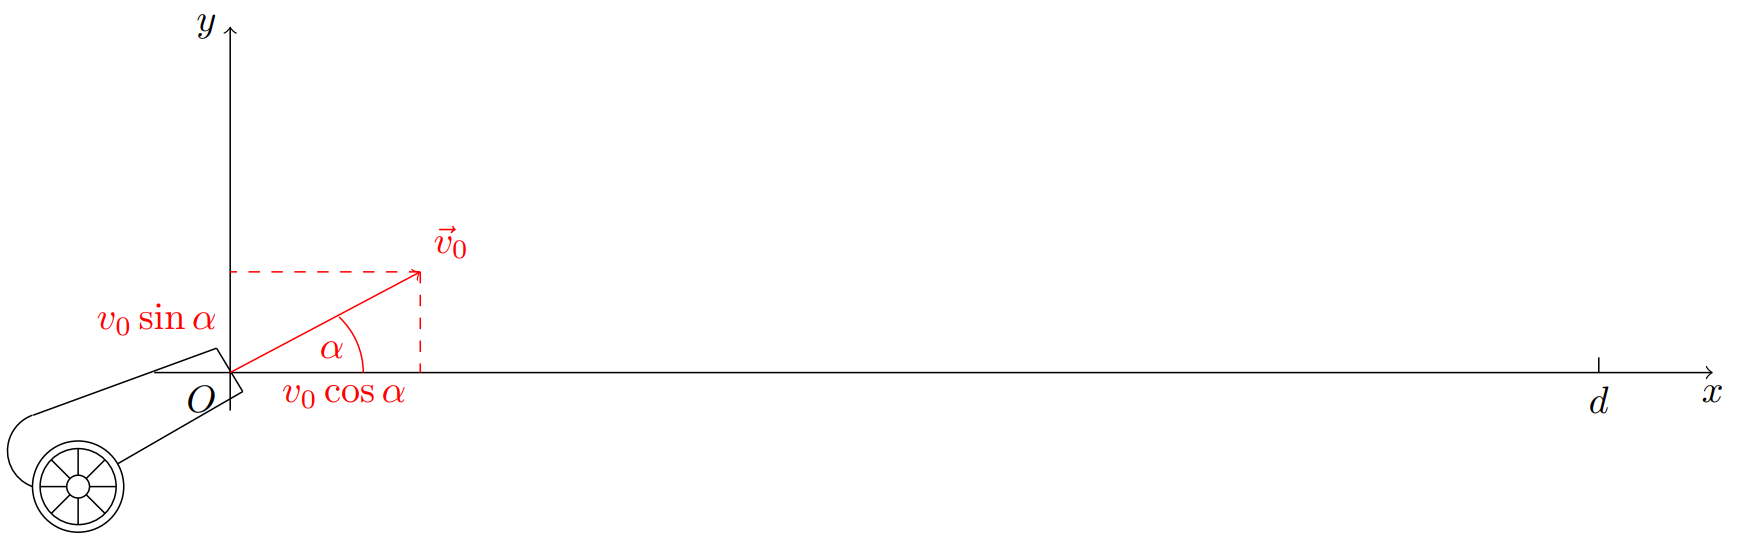
\includegraphics[scale = 0.5]{Images/Canon}
\end{center}
    
\end{frame}
\begin{comment}
\begin{frame}{Balistique : chute libre}
\vspace*{1cm}
    \noindent\begin{minipage}{0.5\textwidth}
 \begin{figure}[H]
    \centering
    
\definecolor{uuuuuu}{rgb}{0.26666666666666666,0.26666666666666666,0.26666666666666666}
\begin{tikzpicture}[line cap=round,line join=round,>=triangle 45,x=1.0cm,y=1.0cm]
\draw (5,7) node{$m\vec a = m\vec g \iff m\ddot x\vec e_x = -mg \vec e_x $};
\draw (5.2,6.3) node{$\iff \ddot x = -g$};
\draw (3.65,5.6) node{$\Rightarrow \dot x = -gt+A$};
\draw (4.3,4.9) node{$\Rightarrow x = -\frac{1}{2}gt^2+At+B$};
\draw (4.3,3.5) node{$\dot x(0) = A = v_0$};
\draw (4.3,2.8) node{$x(0) = B = x_0$};
\draw (4.3,1.5) node{$\Rightarrow x(t) = -\frac{1}{2}gt^2+v_0t+x_0$};
\draw [->] (0.05,0.1)--(0.05,1.1);
\draw (0.05,0.6) node[left]{$\vec e_x$};
\begin{axis}[
x=1.0cm,y=1.0cm,
axis y line=middle,
axis x line=none,
ymajorgrids=true,
xmajorgrids=false,
xmin=-0.05,
xmax=1.5,
ymin=-0.1,
ymax=7.0,
xtick={-0.0,2.0},
ytick={-0.0},]
\clip(-0.05,-0.1) rectangle (1.5,7.);
\draw[line width=0.8pt] (-2.8087273377408764,8.902841339382519) -- (0.17459772664676576,8.902841339382519);
\begin{scriptsize}
\draw [fill=black] (0.17459772664676576,8.902841339382519) circle (1.5pt);
\draw[color=black] (0.3237639798661478,9.193715533160313) node {$t = 1.2$};
\draw [fill=uuuuuu] (1.,-0.0032) circle (2.0pt);
\draw[color=uuuuuu] (1.0994284966069348,0.24374033999739933) node {$M$};
\draw[color=uuuuuu] (0.2,6.8) node {$x$};
\draw [fill=uuuuuu] (1.,6.8638) circle (2.0pt);
\draw [fill=uuuuuu] (1.,6.2752) circle (2.0pt);
\draw [fill=uuuuuu] (1.,5.2942) circle (2.0pt);
\draw [fill=uuuuuu] (1.,3.9208) circle (2.0pt);
\draw [fill=uuuuuu] (1.,2.155) circle (2.0pt);
\draw [fill=uuuuuu] (1.,-0.0032) circle (2.0pt);

\end{scriptsize}
\end{axis}
\draw [<-] (-1,4) -- (-1,5);
\draw (-1,4.5) node [left]{$\vec g$};
\end{tikzpicture}
    %\caption{Le point $M$ est en chute libre}
    \label{fig:my_label}
\end{figure}
\vspace{2\baselineskip}
\end{minipage}

%$m\vec a = m\vec \iff mx\vec e_x = -mg \vec e_x \iff m\ddot x = -mg $
\end{frame}




\begin{frame}{Application: Boulet de Canon (I)}
    \begin{gather*}
        m\vec a = m\vec g \Rightarrow \vec a = \vec g \Rightarrow 
    \begin{cases}
      \ddot{x} = 0, & \mbox{ selon l'axe $\mathbf{e}_x$}\\
     \ddot{y} = -g, & \mbox{ selon l'axe $\mathbf{e}_y$}
   \end{cases} \\
   \Rightarrow
   \begin{cases}
      \dot{x} = C\\
     \dot{y} = -gt+A 
   \end{cases} 
   \quad \Rightarrow
   \begin{cases}
      x = Ct+D\\
     y = -\frac{1}{2}gt^2+At+B
   \end{cases} \\ 
    \end{gather*}
    \begin{center}
    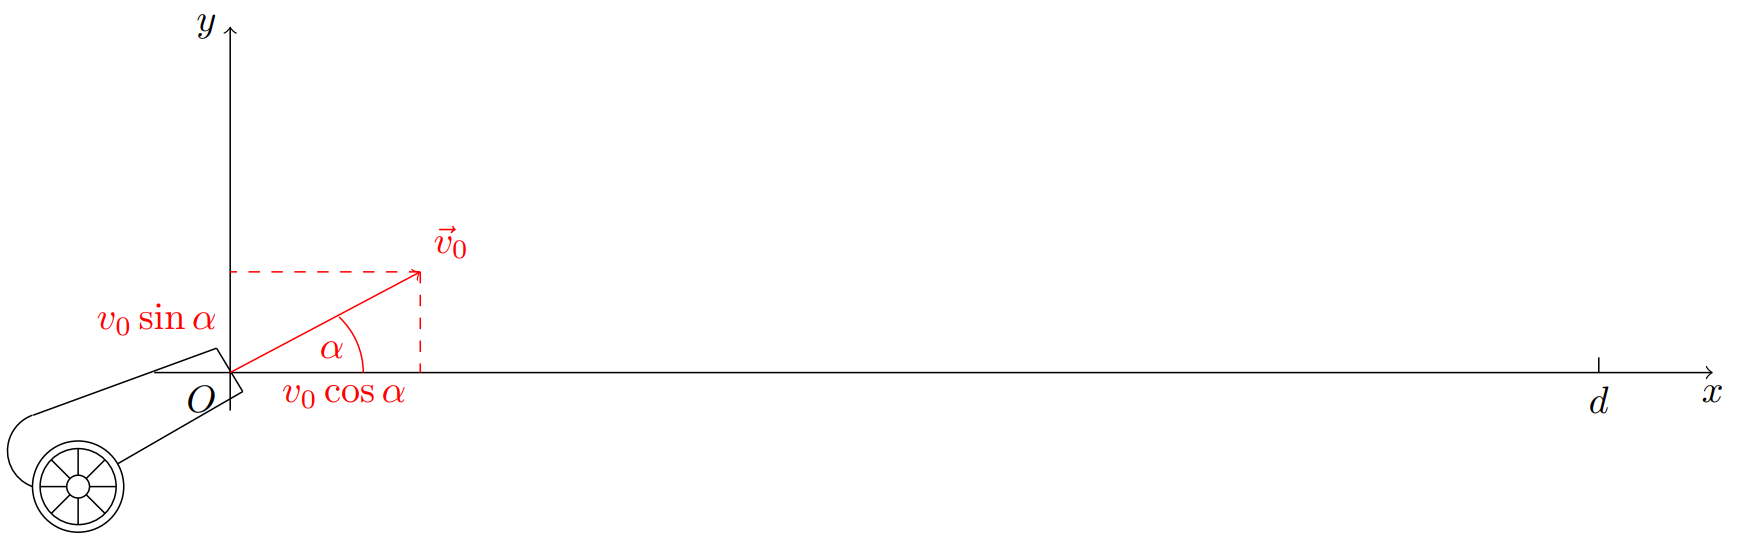
\includegraphics[scale = 0.5]{Images/Canon} \\
    \end{center}
\end{frame}    

\begin{frame}{Application: Boulet de Canon (II)}
\begin{gather*}
   \textrm{Conditions initiales : }  \\
   \begin{cases}
      \dot x(0) = v_0\cos{\alpha}=C\\
     \dot y(0) = v_0\sin{\alpha}=A
   \end{cases} 
   \quad \textrm{et} \quad
   \begin{cases}
      \dot x(0) = 0=D\\
     \dot y(0) = 0=B
   \end{cases}\\
   \Rightarrow 
   \begin{cases}
      x(t) =  v_0\cos{(\alpha)}t\\
    y(t) = -\frac{1}{2}gt^2+v_0\sin{(\alpha)}t
   \end{cases}  
\end{gather*}

\begin{center}
    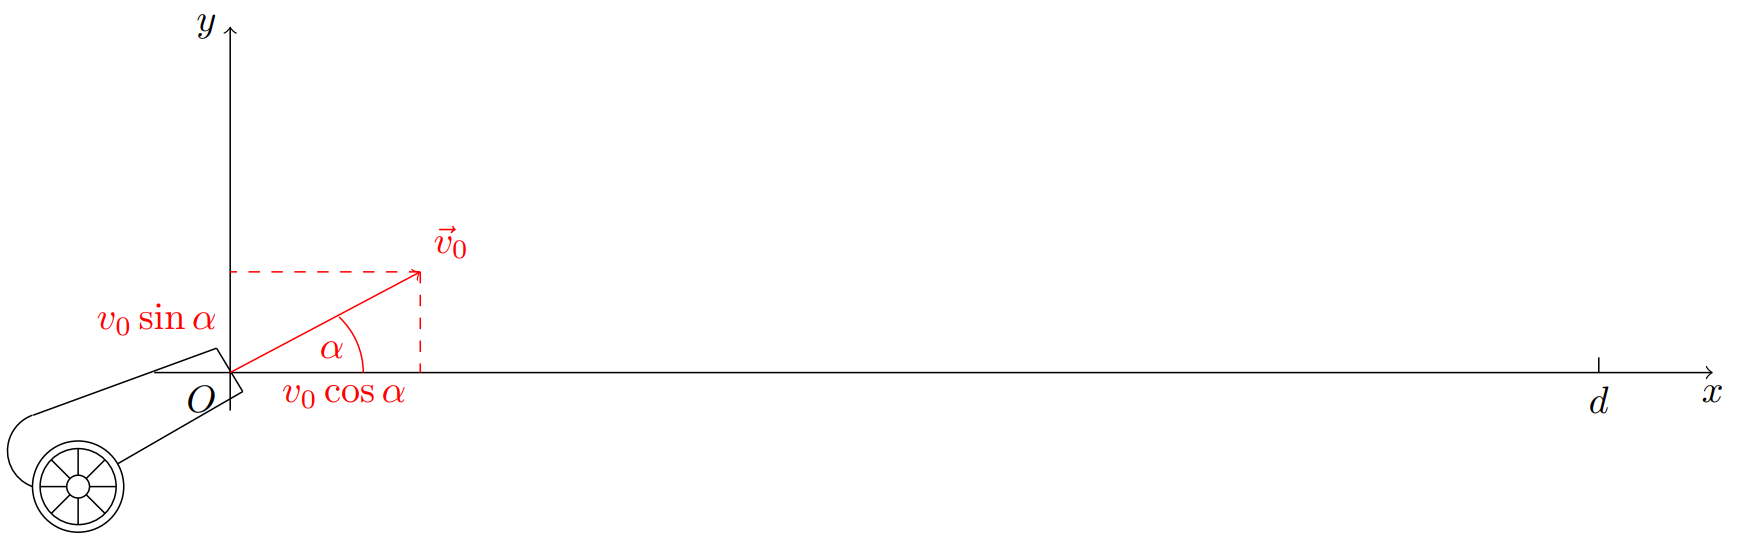
\includegraphics[scale = 0.5]{Images/Canon} \\  
\end{center}
\end{frame}

\begin{frame}{Application: Boulet de Canon (III)}
Soit $t_i$ le temps auquel le boulet atteint l'enceinte. A ce point on a :
\begin{gather*}
 \begin{cases}
      d =  v_0\cos{(\alpha)}t_i\\
    0 = -\frac{1}{2}gt_i^2+v_0\sin{(\alpha)}t_i
   \end{cases} 
   \Rightarrow 
   \begin{cases}
     t_i =  \frac{d}{v_0\cos{(\alpha)}}\\
    -v_0\sin{(\alpha)} \frac{d}{v_0\cos{(\alpha)}} = -\frac{1}{2}g (\frac{d}{v_0\cos{(\alpha)}})^2
   \end{cases} \\
   \textrm{On travaille la deuxième équation pour essayer d'isoler l'angle : }\\
   \Rightarrow 
  v_0\sin{(\alpha)}=  \frac{gd}{2v_0\cos{(\alpha)}}
 \Rightarrow 
  2\cos{(\alpha)}sin{(\alpha)}=  \frac{gd}{{v_0}^2} \\
  sin{(2\alpha)}=\frac{gd}{{v_0}^2} 
\end{gather*}

\begin{center}
    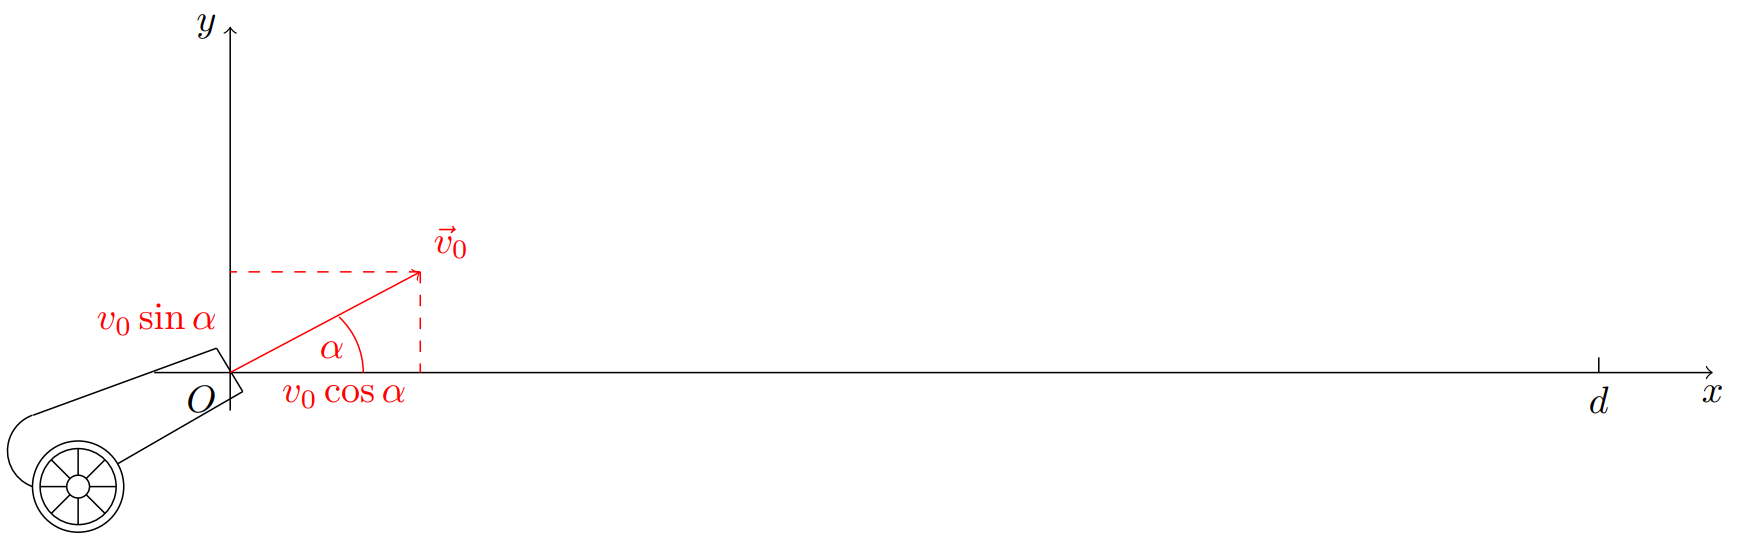
\includegraphics[scale = 0.5]{Images/Canon} \\  
\end{center}
\end{frame}

\begin{frame}{Application: Boulet de Canon (IV)}
 En se rappelant que tout réel dans (-1;1) a deux antécédents entre 0 et $2\pi$ par la fonction sinus, on s'aperçoit qu'il y a en fait deux solutions :
 \begin{equation*}
     \begin{cases}
       \alpha_1 = \frac{1}{2}\arcsin{(\frac{gd}{{v_0}^2} )}\\
       \alpha_2 = \frac{\pi}{2}-\frac{1}{2}\arcsin{(\frac{gd}{{v_0}^2} )}
     \end{cases}
 \end{equation*}
On voit par ailleurs que la fonction arcsin étant défini entre -1 et 1, qu'on doit avoir $v_0^2 \geq gd$.
\begin{center}
    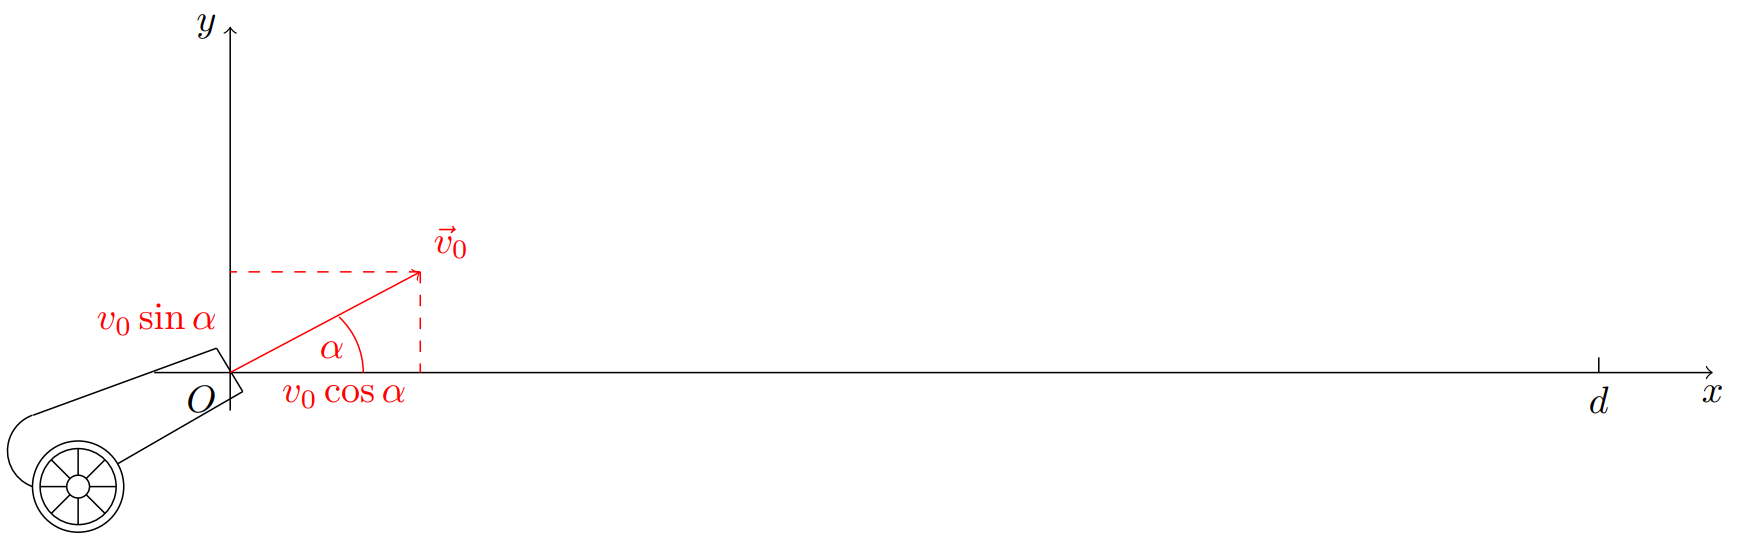
\includegraphics[scale = 0.5]{Images/Canon} \\  
\end{center}
\end{frame}

\begin{frame}{Application: Boulet de Canon (V)}
 On vérifie maintenant l'homogénéité de la solution. Un angle est une grandeur sans unité, chose vérifiée ici comme arcsin retourne une valeur sans dimension. Il ne faut pas oublier de vérifier que $\frac{gd}{{v_0}^2}$ soit sans unité : 
 \begin{equation}
       \left[\frac{gd}{v_{0}^2}\right]= \frac{L}{T^2} \dfrac{L}{\frac{L^2}{T^2}} = 1,
 \end{equation}
On n'a donc pas de problème de dimension !
On vérifie la cohérence de la solution, en faisant tendre par exemple $v_0$ vers l'infini. 
\begin{equation*}
    \lim\limits_{v_0 \rightarrow +\infty} \frac{gd}{v_{0}^2} = 0 \quad \textrm{et} \quad \lim\limits_{x \rightarrow 0} \arcsin{x} = 0
\end{equation*}
Donc : 
\begin{equation*}
    \begin{cases}
        \lim\limits_{v_0 \rightarrow +\infty} \alpha_1 =  \lim\limits_{v_0 \rightarrow +\infty} \frac{1}{2}\arcsin{(\frac{gd}{{v_0}^2} )} = 0\\
        \lim\limits_{v_0 \rightarrow +\infty} \alpha_2 =  \lim\limits_{v_0 \rightarrow +\infty} \frac{\pi}{2}-\frac{1}{2}\arcsin{(\frac{gd}{{v_0}^2} )} = \frac{\pi}{2}
     \end{cases}
\end{equation*}
Ces deux solutions sont cohérentes, on est rassuré, il n'y a pas d'erreur apparente.

\end{frame}


\begin{frame}{Méthodologie de Résolution (1)}
    \begin{enumerate}
    \item Tout d'abord, je vous conseille de faire un schéma de la situation. Faites-y figurer les distances, les angles et les forces que subissent vos objets.
    \item Ensuite, sortez un de vos meilleures outils, la deuxième loi de Newton! Écrivez la relation, puis projeter vos fores. Ensuite vous pourrez décomposer l'accélération selon votre base et identifiez pour chaque composante de l'accélération les forces qui la provoquent. 
    \item Maintenant vous avez des équations différentielles avec comme inconnue l'accélération selon votre base. Si vous pouvez intégrer comme dans notre exemple, faites le pour obtenir les équations horaires. Sinon, peut-être est-ce une équation particulière comme celle de l'oscillateur harmonique et dans ce cas là, il faut que vous donniez la solution que vous connaissez. 
    \item Vous avez vos équations horaires. Maintenant, il faut déterminer vos constantes grâce aux conditions initiales.
    
\end{enumerate}
\end{frame}
\begin{frame}{Méthodologie de Résolution (2)}
\begin{itemize}
\item Et voilà, vous avez gagné! La question peut être de déterminer une variable en fonction des autres comme dans l'exemple. Dans ce cas là, il faut que vous posiez votre système d'équations avec les informations dont vous disposez. 
    \item Finalement, il vous reste à vérifier vos réponses. Le plus souvent on peut le faire en vérifiant l'homogénéité et le comportement aux limites. Parfois, vous pouvez aussi insérer vos solutions dans les équations initiales (si ou vous demande de trouver une équation horaire par exemple). Notez que ces vérifications ne garantissent pas que votre réponse soient correct, mais peut permettre de démasquer certaines erreurs. Bon courage!
    \end{itemize}
\end{frame}


\end{comment}








\end{document}